
\renewcommand{\thefootnote}{\fnsymbol{footnote}}

\title{A GPU implementation of time domain full waveform inversion}

\author{Pengliang Yang\footnotemark[1], Jinghuai Gao\footnotemark[1], and Baoli Wang\footnotemark[2] \\
\footnotemark[1]Xi'an Jiaotong University, National Engineering Laboratory for Offshore Oil Exploration, Xi'an, China, 710049\\
\footnotemark[2]CCTEG  Xi'an Research Institute, Xi'an, China, 710077
}

\usetikzlibrary{decorations.pathreplacing} 
\usetikzlibrary{shapes,arrows,chains}


\righthead{GPU-based FWI}
\lefthead{Yang et al.}

\maketitle

\begin{abstract}
GPU has become a popular programming tool for seismic imaging and inversion due to its superior speedup performance. One key problem for GPU implementation is that the computation is much faster than the data exchange between host and device. In this paper we implement GPU-based full waveform inversion (FWI) using the wavefield reconstruction strategy. The boundaries of the forward modeling are saved on device to avert the issue of CPU-GPU data transfer. The Clayton-Enquist absorbing boundary is utilized to maintain the efficiency of GPU computation. A hybrid nonlinear conjugate gradient method is adopted in the FWI optimization.  The parallel reduction algorithm is deployed to do computation on GPU blocks. The numerical results demonstrate the validity of our GPU implementation. 

\end{abstract}


\section{Introduction}

Time domain full waveform inversion (FWI) was proposed by \cite{tarantola1984inversion} to refine the velocity model, and developed by   \cite{tarantola1986strategy} and \cite{pica1990nonlinear} as well as many others. Later, frequency domain FWI was proposed by Pratt and Shin in \cite{pratt1998gauss}. In recent years, the Laplace domain FWI and the Laplace-Fourier domain variant have also been developed by \cite{shin2008waveform,shin2009waveform}. Until now, building a good velocity model is still a chanllenging problem and gains increasing effort of geophysicists. 

There are many drawbacks in FWI, such as the non-linearity, the non-uniqueness of the solution, as well as the expensive computational cost. The goal of FWI is to match the synthetic and the observed data.
The minimization of the misfit function is essentially an iterative, computation intensive procedure: at each iteration one has to calculate the derivative of the objective function with respect to the model parameters by cross correlating the back propagated residual wavefield with the corresponding forward source propagated wavefield. The forward modeling itself demands large computational effort, while back propagated residual wavefield begs for large memory requirement to store the source wavefield. 

Recent advances in computing capability and hardware makes FWI a popular research subject to improve velocity models. As a booming technology, graphics processing unit (GPU) has been widely used to mitigate the computational drawbacks in seismic imaging \citep{micikevicius20093d} and inversion \citep{boonyasiriwat2010multisource,shin20143d}, due to its superior speedup performance. 
One key problem for GPU implementation is that the computation is much faster while the data exchange between host and device always takes longer time.  This paper is devoted to the implementation of  GPU-based FWI using the wavefield reconstruction strategy. The boundaries of the forward modeling are saved on device to avert the issue of CPU-GPU data transfer. Shared memory is used to speedup the modeling computation. A hybrid nonlinear conjugate gradient method is adopted in the FWI optimization.  In each iteration, a Gaussian shaping step is employed to remove the outliers in of the computed gradient. Instead of solving industrial scale problem, we demonstrate the validity and the relatively superior speedup of our GPU implementation for 2D study.


\section{FWI and its GPU implementation}

\subsection{FWI: data mismatch minimization}

In the case of constant density, the acoustic wave equation is specified by
\begin{equation}\label{eq:acoustic}
\frac{1}{v^2(\textbf{x})}\frac{\partial^2 p(\textbf{x},t;\textbf{x}_s)}{\partial t^2}-\nabla^2 p(\textbf{x},t;\textbf{x}_s)=f_s(\textbf{x},t;\textbf{x}_s).
\end{equation}
where $ f_s(\textbf{x},t;\textbf{x}_s)=f(t')\delta(\textbf{x}-\textbf{x}_s)\delta(t-t')$. 
According to the above equation, a misfit vector  $\Delta \textbf{p}=\textbf{p}_{cal}-\textbf{p}_{obs}$ is given by the differences at the receiver positions between the recorded seismic data $\textbf{p}_{obs}$ and the modeled seismic data $\textbf{p}_{cal}=\textbf{f}(\textbf{m})$ for each source-receiver pair of the seismic survey. Here, in the simplest acoustic velocity inversion, $\textbf{f}(\cdot)$ indicates the forward modeling process while $\textbf{m}$ corresponds to the velocity model to be determined. The goal of FWI is to match the data misfit by iteratively updating the velocity model. The objective function taking the least-squares norm of the misfit vector $\Delta \textbf{p}$ is given by
\begin{equation}\label{eq:obj}
E(\textbf{m})=\frac{1}{2}\Delta \textbf{p}^{\dagger}\Delta \textbf{p}
=\frac{1}{2}\|\textbf{p}_{cal}-\textbf{p}_{obs}\|^2
=\frac{1}{2}\sum_{r=1}^{ng}\sum_{s=1}^{ns}\int_{0}^{t_{\max}}\mathrm{d}t|p_{cal}(\textbf{x}_r, t;\textbf{x}_s)-p_{obs}(\textbf{x}_r, t;\textbf{x}_s)|^2
\end{equation}
where $ns$ and $ng$ are the number of sources and geophones/receivers, $\dagger$ denotes the adjoint operator (transpose conjugate), and $\textbf{f}(\cdot)$ indicates the forward modeling of the wave propagation. The recorded seismic data is only a small subset of the whole wavefield.

The gradient-based minimization method updates the velocity model according to a descent direction $\textbf{d}_k$:
\begin{equation}\label{eq:cg}
\textbf{m}_{k+1}=\textbf{m}_k+\alpha_k \textbf{d}_k.
\end{equation}
where $k$ denotes the iteration number. By neglecting the terms higher than the 2nd order, the objective function can be expanded as
\begin{equation}
E(\textbf{m}_{k+1})=E(\textbf{m}_k+\alpha_k \textbf{d}_{k})=E(\textbf{m}_k)+\alpha_k \langle\nabla E(\textbf{m}_k),\textbf{d}_k\rangle+\frac{1}{2}\alpha_k^2\textbf{d}_k^{\dagger}\textbf{H}_k\textbf{d}_k.
\end{equation}
Differentiation the misfit function $E(\textbf{m}_{k+1})$ with respect to $\alpha_k$ gives
\begin{equation}\label{eq:alpha1}
\alpha_k=-\frac{\langle\textbf{d}_k,\nabla E(\textbf{m}_k)\rangle}{\textbf{d}_k^{\dagger}\textbf{H}_k\textbf{d}_k}
=-\frac{\langle\textbf{d}_k,\nabla E(\textbf{m}_k)\rangle}{\langle\textbf{J}_k\textbf{d}_k,\textbf{J}_k\textbf{d}_k\rangle}
=\frac{\langle\textbf{J}_k\textbf{d}_k,\textbf{p}_{obs}-\textbf{p}_{cal}\rangle}{\langle\textbf{J}_k\textbf{d}_k,\textbf{J}_k\textbf{d}_k\rangle}
\end{equation}
in which we use the approximate Hessian $\textbf{H}_k:=\textbf{H}_a=\textbf{J}_k^{\dagger}\textbf{J}_k$ and $\nabla_{\textbf{m}}E=\textbf{J}^{\dagger}\Delta \textbf{p}$, according to equation \eqref{eq:grad}. A detailed derivation of the minimization process is given in Appendix A.


\subsection{Nonlinear conjugate gradient method}

The conjugate gradient (CG) algorithm decreases the misfit function along the conjugate gradient direction:
\begin{equation}
	\textbf{d}_k=
	\begin{cases}
	-\nabla E(\textbf{m}_0), & k=0\\
	-\nabla E(\textbf{m}_k)+\beta_k \textbf{d}_{k-1}, & k\geq 1
	\end{cases}
\end{equation}
There are a number of ways to compute $\beta_k$. I use a hybrid a hybrid scheme combing Hestenes-Stiefel method and Dai-Yuan method  \citep{hager2006survey}
\begin{equation}
\beta_k=\max(0, \min(\beta_k^{HS},\beta_k^{DY})).
\end{equation}
in which
\begin{equation}\label{eq:beta}
\left\{
\begin{split}
\beta_k^{HS}&=\frac{\langle\nabla E(\textbf{m}_k),\nabla E(\textbf{m}_k)-\nabla E(\textbf{m}_{k-1})\rangle}{\langle\textbf{d}_{k-1},\nabla E(\textbf{m}_k)-\nabla E(\textbf{m}_{k-1})\rangle}\\
\beta_k^{DY}&=\frac{\langle\nabla E(\textbf{m}_k),\nabla E(\textbf{m}_k)\rangle}{\langle\textbf{d}_{k-1},\nabla E(\textbf{m}_k)-\nabla E(\textbf{m}_{k-1})\rangle}
\end{split}
\right.
\end{equation}
This provides an automatic direction reset while avoiding over-correction of $\beta_k$ in conjugate gradient iteration. It reduces to steepest descent method when the subsequent search directions lose conjugacy. The gradient of the misfit function w.r.t. the model is given by \citep{bunks1995multiscale}
\begin{equation}
\nabla E_{\mathrm{m}}
=\frac{2}{v^3(\textbf{x})}\sum_{r=1}^{ng}\sum_{s=1}^{ns}\int_{0}^{t_{\max}}\mathrm{d}t 
\frac{\partial^2 p_{cal}(\textbf{x},t;\textbf{x}_s)}{\partial t^2}p_{res}(\textbf{x}_r,t;\textbf{x}_s)\\
\end{equation}
where $p_{res}(\textbf{x},t;\textbf{x}_s)$ back propagated residual wavefield, see the Appendix B and C for more details. A Gaussian smoothing operation plays an important role in removing the outliers for the computed gradient. To obtain a reasonable step size $\alpha_k$ according to equation \eqref{eq:alpha1}, we estimate a small step length $\epsilon$ proposed in \cite{pica1990nonlinear}:
\begin{equation}
\max(\epsilon |\textbf{d}_k|)\leqslant \frac{\max(|\textbf{m}_k|)}{100}.
\end{equation}
and the Taylor approximation
\begin{equation}
\textbf{J}_k\textbf{d}_k\approx\frac{\textbf{f}(\textbf{m}_k+\epsilon \textbf{d}_k)-\textbf{f}(\textbf{m}_k)}{\epsilon}
\end{equation}
We summarize the FWI flowchart in Figure~\ref{fig:flowchart}.


% Define block styles
\tikzstyle{decision} = [diamond, draw, fill=blue!20, 
    text width=4.5em, text badly centered, node distance=2.8cm, inner sep=0pt]
\tikzstyle{block} = [rectangle, draw, fill=blue!20, 
    text width=14em, text centered, rounded corners, minimum height=2em]
\tikzstyle{blocksmall} = [rectangle, draw, fill=blue!20, node distance=4cm,
    text width=6em, text centered, rounded corners, minimum height=2em]
\tikzstyle{line} = [draw, -latex']

\begin{figure}
  \centering 
\begin{tikzpicture}[node distance = 3.5cm, auto]
    % Place nodes
    \node [blocksmall] (init) {initialize with starting model};
    \node [decision, below of=init] (iter) {k$<$niter?};
    \node [blocksmall, left of=iter](output) {output FWI result};   
    \node [block, below of=iter] (forw) {1)generate synthetic seismogram via modeling, 2) save the effective boundaries, and 3) compute the residual wavefield};
    \node [block, below of=forw] (back) {1)reconstruct source wavefield with saved boundaries, 2)back propagate residual wavefield, and 3) calculate the gradient}; 
    \node [decision, below of=back] (is) {is$<$ns?};
    \node [blocksmall,left of=is] (loop) {loop over shots: is++};
    \node [blocksmall, right of=is] (cg) {calculate $\beta_k$ and the conjugate gradient};
    \node [blocksmall, right of=cg] (eps) {estimate trial stepsize $\epsilon$ and a test velocity};
    \node [blocksmall, above of=eps] (est) {estimate stepsize $\alpha_k$: redo forward modeling (ns shots)};
    \node [blocksmall, above of=est] (update) {update velocity model, k++};
    % Draw edges
    \path [line] (init) -- (iter);
    \path [line] (iter) --node [near start] {Yes} (forw);
    \path [line] (forw) -- (back);
    \path [line] (back) -- (is);
    \path [line] (is) --node [near start] {Yes} (loop);
    \path [line] (loop) |- (forw);
    \path [line] (is)--node[near start]{No} (cg);
    \path [line] (cg)--(eps);
    \path [line] (eps)--(est);
    \path [line] (est)--(update);
    \path [line] (update)|-(iter);
    \path [line] (iter)--node[near start]{No}(output);
\end{tikzpicture}
  \caption{The flowchart of FWI}\label{fig:flowchart}
\end{figure}

\subsection{Wavefield reconstruction via boundary saving}

One key problem of GPU-based RTM is that the computation is much faster while the data exchange between host and device always takes longer time. Many researchers choose to reconstruct the source wavefield instead of storing the modeling time history on the disk, just saving the boundaries \citep{dussaud2008computational,Yang201464}. For $2N$-th order finite difference, regular grid scheme needs to save $N$ points on each side \citep{dussaud2008computational}, while staggered-grid scheme required at least $2N-1$ points on each side \citep{Yang201464}. In our implementation, we use 2nd order regular grid finite difference because FWI begins with a rough model and velocity refinement is mainly carried out during the optimization. Furthermore, high order finite difference and staggered-grid schemes does not necessarily leads to FWI converge to an accurate solution while asking for more computational cost. A key observation for wavefield reconstruction is that one can reuse the same template by exchanging the role of $p^{k+1}$ and $p^{k-1}$. In other words, for forward modeling we use
\begin{equation}\label{eq:forward}
p^{k+1}=2p^{k}-p^{k-1}+v^2\Delta t^2 \nabla^2 p^{k}.
\end{equation}
while for backward reconstruction we use
\begin{equation}\label{eq:backward}
p^{k-1}=2p^{k}-p^{k+1}+v^2\Delta t^2 \nabla^2 p^{k}.
\end{equation}
The wavefield extrapolation can be stepped efficiently via pointer swap, i.e.,
\begin{equation}
\begin{split}
 &for\;ix,iz... \quad p_0(:)=2p_1(:)-p_0(:)+v^2(:)\Delta t^2 \nabla^2 p_1(:)\\
 &ptr=p_0;p_0=p_1;p_1=ptr;// \mathrm{swap\; pointer}
\end{split}
\end{equation}
where $(:)=[ix,iz]$, $p_0$ and $p_1$ are $p^{k+1}/p^{k-1}$ and $p^k$, respectively. 


Note that all the computation is done on GPU blocks. In our codes, the size of the block is set to be 16x16. We pad the velocity model to be mutiple of 16x16 in order to coalesce thread loads. As shown in Figure~\ref{fig:blocks}, the whole computation area are divided into 16x16 blocks. For each block, we use a 18x18 shared memory array to cover all the grid points in this block. It implies that we add a redundant point on each side, which stores the value from other blocks, as marked by the window in Figure~\ref{fig:blocks}.  When the computation is not performed for the interior blocks, special care needs to be paid to the choice of absorbing boundary condition (ABC) in the design of FWI codes. Allowing for efficient GPU implementation, we use the $45^o$ Clayton-Enquist ABC proposed in \cite{clayton1977absorbing} and \cite{engquist1977absorbing}. For the left boundary, it is
\begin{equation}
 \frac{\partial^2 p}{\partial x\partial t}-\frac{1}{v}\frac{\partial^2 p}{\partial t^2}=\frac{v}{2}\frac{\partial^2 p}{\partial z^2}
\end{equation}
which requires only one layer to be saved on each side for wavefield reconstruction. The equations for right and bottom boundary can also be written in a similar way. To simulate free surface boundary condition, no ABC is applied to the top boundary. It is interesting to note that the same tenique has been adopted by \cite{liu2013wavefield} for reverse time migration. We believe its application to FWI is straightforward and more valuable.


\begin{figure}
  \centering
  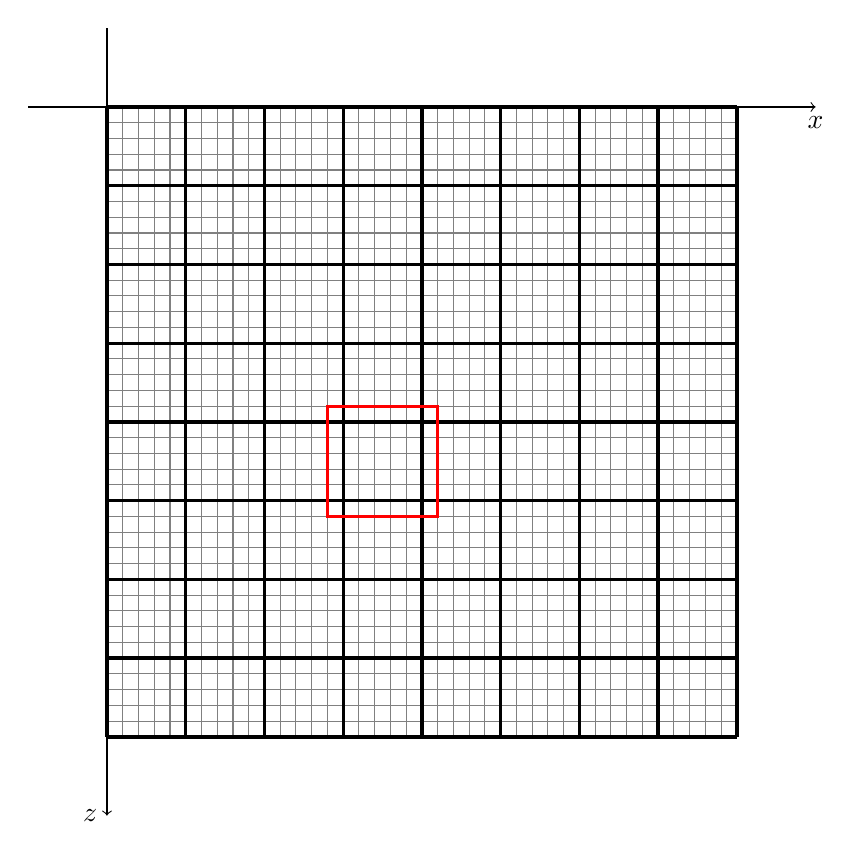
\begin{tikzpicture}
    % Draw x and y axis lines
    \draw [->] (-5,4) -- (5,4) node [below] {$x$};
    \draw [->] (-4,5) -- (-4,-5) node [left] {$z$};
    \draw[step=0.2cm,color=gray] (-4,-4) grid (4,4);   
    \draw[very thick] (-4,-4)--(-4,4);
    \draw[very thick] (4,-4)--(4,4);
    \draw[very thick] (3,-4)--(3,4);
    \draw[very thick] (2,-4)--(2,4);
    \draw[very thick] (1,-4)--(1,4);
    \draw[very thick] (0,-4)--(0,4);
    \draw[very thick] (-3,-4)--(-3,4);
    \draw[very thick] (-2,-4)--(-2,4);
    \draw[very thick] (-1,-4)--(-1,4);
    \draw[very thick] (-4,-4)--(4,-4);
    \draw[very thick] (-4,-3)--(4,-3);
    \draw[very thick] (-4,-2)--(4,-2);
    \draw[very thick] (-4,-1)--(4,-1);
    \draw[very thick] (-4,0)--(4,0);
    \draw[very thick] (-4,4)--(4,4);
    \draw[very thick] (-4,3)--(4,3);
    \draw[very thick] (-4,2)--(4,2);
    \draw[very thick] (-4,1)--(4,1);    
    \draw [very thick,red] (-1.2,-1.2) rectangle (0.2,0.2);    
  \end{tikzpicture}
  \caption{2D blocks in GPU memory. The marked window indicates that the shared memory in every block needs to be extended on each side with halo cells which stores the grid value from other blocks.}\label{fig:blocks}
\end{figure}


\subsection{Parallel reduction on CUDA blocks}

Recognizing that  hardware serializes divergent thread execution within same warp whereas all threads of warp have to complete execution before warp ends, we use parallel reduction technique to find the maximum of model vector $\max(\textbf{m}_k)$ and the descent vector $\max(\textbf{d}_k)$, as well as the inner product in the numerator and the denominator of $\alpha_k$. 
A sequential addressing scheme is utilized because it is free of conflict\citep{harris2007optimizing}. As shown in Figure~\ref{fig:reduction}, in each level half of the threads will perform the reading from global memory and writing to shared memory. The required number of threads will decrease to be half of the previous level. Theoretically, this kind of parallel reduction reduces original computational complexity $O(N)$ to be $O(\log_2(N))$, which may bring significant improvement in computational efficiency. 


\begin{figure}
\centering
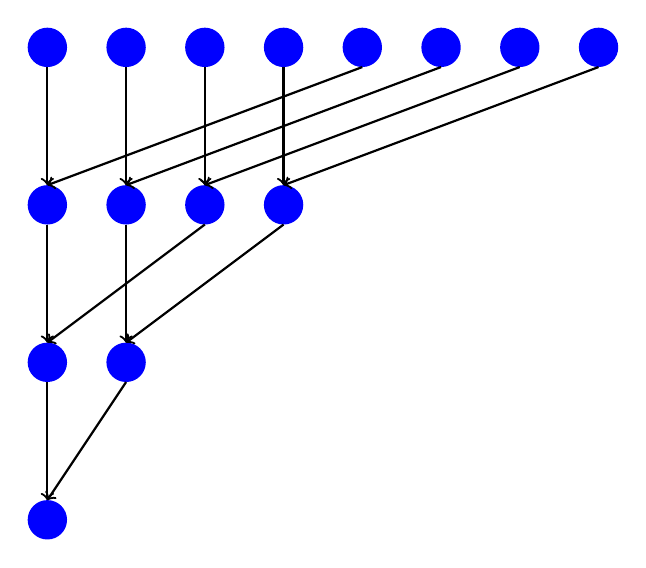
\begin{tikzpicture}
  \fill[semithick,blue] (0,0)  circle (0.25) (1,0) circle(0.25)  (2,0) circle(0.25)   (3,0) circle(0.25) 
  (4,0) circle(0.25) (5,0) circle(0.25) (6,0) circle(0.25) (7,0) circle(0.25); 
  \fill [semithick,blue] (0,-2)  circle (0.25) (1,-2) circle(0.25)  (2,-2) circle(0.25)   (3,-2) circle(0.25);  
  \draw[thick,->] (0,-0.25)--(0,-1.75);
  \draw[thick,->] (4,-0.25)--(0,-1.75);  
  \draw[thick,->] (1,-0.25)--(1,-1.75);
  \draw[thick,->] (5,-0.25)--(1,-1.75);
  \draw[thick,->] (2,-0.25)--(2,-1.75);
  \draw[thick,->] (6,-0.25)--(2,-1.75);  
  \draw[thick,->] (3,-0.25)--(3,-1.75);
  \draw[thick,->] (7,-0.25)--(3,-1.75);
  
  \fill [semithick,blue] (0,-4) circle (0.25) (1,-4) circle(0.25); 
  \draw[->] (2,-0.25)--(2,-1.75); 
  \draw[thick,->] (0,-2.25)--(0,-3.75);
  \draw[thick,->] (2,-2.25)--(0,-3.75);  
  \draw[thick,->] (1,-2.25)--(1,-3.75);
  \draw[thick,->] (3,-2.25)--(1,-3.75);
  
  \fill [semithick,blue] (0,-6) circle (0.25);
  \draw[thick,->] (0,-4.25)--(0,-5.75);
  \draw[thick,->] (1,-4.25)--(0,-5.75);
\end{tikzpicture}
\caption{Parallel reduction on GPU blocks using a sequential addressing scheme}\label{fig:reduction}
\end{figure}



\section{Numerical results}

\subsection{Exact reconstruction with saved boundaries}
\inputdir{fbrec}

Since we are advocating the wavefield reconstruction method in FWI, the foremost thing is to demonstrate that the boundary saving strategy does not introduce any kind of error/artifacts for the wavefield to be reconstructed. To attain this goal, we design a constant velocity model: velocity=2000 m/s, $nz=nx=200$, $\Delta z=\Delta x=5m$. The 15Hz Ricker wavelet is taken as the source and set at the center of the model. We do the modeling process for 1000 steps with time interval $\Delta=1$ms. We record the modeled wavefield snap at 0.28s and 0.4s, as shown in the top panels of Figure~\ref{fig:fb}. It is shown that at time 0.4s, the wavefield has already spead to the boundaries which absorb most of the reflection energy. In the backward steps, the reconstructed wavefield at 0.4s and 0.28s are also recorded, shown in the bottom panels of Figure~\ref{fig:fb}. As can been seen from the figure, the backward reconstruction starts from the boudaries (bottom left) and gradually recovers the interior wavefield precisely (bottom right). 


\plot{fb}{width=\textwidth}{Backward reconstruction can be realized using the saved boundaries. Note that no absorbing boundary condition is applied on the top boundary of the model in the forward modeling.}

\subsection{Speedup performance}
\inputdir{speedup}

The acceleration of GPU implementation on advanced computer hardware is a key concern of many researchers. There are many factors which may accelerate the FWI computation. Compared with saving the wavefield on the disk, wavefield reconstruction will accelerate the GPU computing because no CPU-GPU data transfer is needed any more. The parallel reduction to find the maxium value of model vector $\textbf{m}_k$ and descent direction vector $\textbf{d}_k$ is another factor to speedup the FWI computation. However, among these factors, the forward modeling takes most of the computing time. In each iteration needs four times of forward modeling: two of them are for sources and receivers; one is performed for wavefield reconstruction and gradient calculation, and another one is to estimate the step length $\alpha_k$. Thus, we focus on the speedup obtained in the forward modeling procedure.

To do the performance analysis fairly, we run the sequential implementation CPU code and parallel multi-thread GPU code of forward modeling for 1000 time steps. We estimate the average time cost of 5 shots for different data size. Because the GPU block size is set to be 16x16. To make the comparison fair, we make the size of the test model to be multiple 16x16. Therefore,  the size of the test model is choosen to be $nx\cdot nz$, $nx=nz=i\cdot160$, where $i=1,\ldots,7$ is an integer. 
Unfortunately, we only have a NVS5400 GPU card (compute capability 2.1, GDDR3) run on a laptop. Even so, compared with sequential implementation on host, we still achieve approximately 2.5--3 times speedup on CUDA device, as shown in Figure~\ref{fig:timecost}. 

\plot{timecost}{width=0.6\textwidth}{Comparison of the time cost for CPU- vs. GPU implementation under  different model size with one shot, 1000 time steps of forward modeling.}



\subsection{Marmousi model}

We use the Marmousi model for the benchmark test, as shown in the top panel of Figure~\ref{fig:marm}.
FWI tacitly requires a good starting model incorporated with low frequency information. Therefore, we use a starting model (bottom panel of Figure~\ref{fig:marm}) obtained by smoothing the original model 20 times with a 5x5 window.

The FWI is carried out for 300 iterations. We record all the updated velocity to make sure the velocity refinement is going on during the iterative procedure. The updated velocity model at the iteration 1, 20, 50, 100, 180 and 300 are displyed in Figure~\ref{fig:vsnap}. Figure~\ref{fig:objs} describes the decreasing misfit function in iterations. As can be seen from the Figures~\ref{fig:vsnap} and \ref{fig:objs}, the velocity model changes significantly at the early stage. Later iterations in FWI make some improvement on small details for the velocity model.


\inputdir{marmtest}

\plot{marm}{width=0.8\textwidth}{Top: The original Marmousi is downsampled with a factor of 3 along depth and lateral direction. The shots are generated according to the subsampled Marmousi model. Bottom: The starting model of FWI for Marmousi model, which is obtained by smoothing the original model 20 times with a 5x5 window.}

\plot{shotsnap}{width=0.8\textwidth}{21 shots were deployed in the FWI. Here, shot 4, 11 and 17 are shown from left to right}

\plot{vsnap}{width=\textwidth}{The updated velocity model at the iteration 1, 20, 50, 100, 180 and 300. }
\plot{objs}{width=0.7\textwidth}{The misfit function decreases with the iterations.}


\section{Conclusions and discussions}

In this paper  we implemented GPU-based FWI using the wavefield reconstruction strategy, which averts the issue of CPU-GPU data transfer. The Clayton-Enquist absorbing boundary was utilized to maintain the efficiency of GPU computation. A hybrid nonlinear conjugate gradient method combined with parallel reduction technique was adopted in the FWI optimization. The validity of our  implementation for GPU-based FWI was demonstrated using numerical test. 

It is important to point out that FWI can be accelerated in many ways. A good choice of preconditioning operator may leads to fast convergence rate and geologically consistent result \citep{virieux2009overview,ayeni2009joint,guitton2012constrained}. Multishooting and source encoding method is also a possible solution for inexpensive FWI \citep{schiemenz2013accelerated,moghaddam2013new}. These techniques can be combined with GPU implementation \cite{wang2011cuda}. There are many reports advocating their acceleration performance based on particular CUDA hardware. These reports may be out of date soon once the more powerful and advanced GPU product are released. Although the speedup performance may be a little poor due to our hardware condition, we believe that compared to chasing a number of reports easy to be obsolete, a better solution is to give readers the implementation code to do performance analysis using their own GPU card. The current GPU-based FWI implementation parallelizes the forward modeling processing which makes it possible to run the FWI on single node and low-level GPU condition even for a laptop. However, it  is completely possible to otain higher speedup performance using the latest, high performance GPU product, and further parallelize the code on multi-GPU architecture using message passing interface (MPI) programming, which will be our subject in the near future. 

\section*{Acknowledgments}

The work of the first author is supported by China Scholarship Council during his visit to The University of Texas at Austin. 
This work is sponsored by National Science Foundation of China (No. 41390454).We wish to thank Sergey Fomel for valuable help to incorporate the codes into Madagascar software package \citep{m8r} (\url{http://www.ahay.org}), which makes all the numerical examples reproducible.


\append{Misfit function minimization}\label{app:misfit}

Here, we mainly follow the delineations of FWI by \cite{pratt1998gauss} and  \cite{virieux2009overview}.The minimum of the misfit function $E(\textbf{m})$ is sought in the vicinity of the starting model $\textbf{m}_0$. The FWI is essentially a local optimization.
In the framework of the Born approximation, we assume that the updated model $\textbf{m}$ of dimension $M$ can be written as the sum of the starting model $\textbf{m}_0$ plus a perturbation model $\Delta \textbf{m}$: $\textbf{m}=\textbf{m}_0+\Delta \textbf{m}$. In the following, we assume that $\textbf{m}$ is real valued.

A second-order Taylor-Lagrange development of the misfit function in the vicinity of $\textbf{m}_0$ gives the expression
\begin{equation}
E(\textbf{m}_0+\Delta \textbf{m})=E(\textbf{m}_0)
+\sum_{i=1}^M\frac{\partial E(\textbf{m}_0)}{\partial m_i}\Delta m_i
+\frac{1}{2}\sum_{i=1}^M\sum_{j=1}^M \frac{\partial^2 E(\textbf{m}_0)}{\partial m_i \partial m_j}\Delta m_i \Delta m_j+O(||\Delta\textbf{m}||^3)
\end{equation}
Taking the derivative with respect to the model parameter $m_i$ results in
\begin{equation}
\frac{\partial E(\textbf{m})}{\partial m_i}=\frac{\partial E(\textbf{m}_0)}{\partial m_i}+\sum_{j=1}^M \frac{\partial^2 E(\textbf{m}_0)}{\partial m_j \partial m_i}\Delta m_j,
i=1,2,\ldots,M.
\end{equation}
Briefly speaking, it is
\begin{equation}
\frac{\partial E(\textbf{m})}{\partial \textbf{m}}=\frac{\partial E(\textbf{m}_0)}{\partial \textbf{m}}+\frac{\partial^2 E(\textbf{m}_0)}{\partial\textbf{m}^2}\Delta \textbf{m}
\end{equation}
Thus,
\begin{equation}\label{eq:deltam}
\Delta \textbf{m}=-\left(\frac{\partial^2 E(\textbf{m}_0)}{\partial\textbf{m}^2}\right)^{-1}\frac{\partial E(\textbf{m}_0)}{\partial \textbf{m}}=-\textbf{H}^{-1}\nabla E_{\textbf{m}}
\end{equation}
where 
\begin{equation}
\nabla E_{\textbf{m}}=\frac{\partial E(\textbf{m}_0)}{\partial \textbf{m}}=\left[
\frac{\partial E(\textbf{m}_0)}{\partial m_1},
\frac{\partial E(\textbf{m}_0)}{\partial m_2},
\ldots,
\frac{\partial E(\textbf{m}_0)}{\partial m_M}\right]^T
\end{equation}
and
\begin{equation}
\textbf{H}=\frac{\partial^2 E(\textbf{m}_0)}{\partial\textbf{m}^2}
=\left(\frac{\partial^2 E(\textbf{m}_0)}{\partial m_i\partial m_j}\right)
\end{equation}
$\nabla E_{\textbf{m}}$ and $\textbf{H}$ are the gradient vector and the Hessian matrix, respectively.


\begin{equation}\label{eq:grad}
\nabla E_{\textbf{m}}=\nabla E(\textbf{m})=\frac{\partial E(\textbf{m})}{\partial \textbf{m}}
=\mathtt{Re}\left[\left(\frac{\partial \textbf{f}(\textbf{m})}{\partial \textbf{m}}\right)^{\dagger}\Delta \textbf{p}\right]
=\mathtt{Re}\left[\textbf{J}^{\dagger}\Delta \textbf{p}\right]
\end{equation}
where $\mathtt{Re}$ takes the real part, and $\textbf{J}=\frac{\partial \textbf{f}(\textbf{m})}{\partial \textbf{m}}$ is the Jacobian matrix, i.e., the sensitivity or the Fréchet derivative matrix.


In matrix form
\begin{equation}\label{eq:descent2}
\textbf{H}=\frac{\partial^2 E(\textbf{m})}{\partial \textbf{m}^2}=\mathtt{Re}\left[\textbf{J}^{\dagger}\textbf{J}\right]+
\mathtt{Re}\left[\frac{\partial \textbf{J}^T}{\partial \textbf{m}^T}(\Delta \textbf{p}^*, \Delta \textbf{p}^*, \ldots, \Delta \textbf{p}^*)\right].
\end{equation}
Most of the time, this second-order term is neglected for nonlinear inverse problems. In the following, the remaining term in the Hessian, i.e., $\textbf{H}_a=\mathtt{Re}[\textbf{J}^{\dagger}\textbf{J}]$, is referred to as the approximate Hessian. It is the auto-correlation of the derivative wavefield. Equation \eqref{eq:deltam} becomes
\begin{equation}
\Delta \textbf{m}
=-\textbf{H}^{-1}\nabla E_{\textbf{m}}
=-\textbf{H}_a^{-1}\mathtt{Re}[\textbf{J}^{\dagger}\Delta \textbf{p}].
\end{equation}

The method which solves equation \eqref{eq:descent2} when only $\textbf{H}_a$ is estimated is referred to as the Gauss-Newton method. To guarantee th stability of the algorithm (avoiding the singularity), we can use $\textbf{H}=\textbf{H}_a+\eta \textbf{I}$, leading to
\begin{equation}\label{eq:hessian}
\Delta \textbf{m}
=-\textbf{H}^{-1}\nabla E_{\textbf{m}}
=-(\textbf{H}_a+\eta \textbf{I})^{-1}\mathtt{Re}\left[\textbf{J}^{\dagger}\Delta \textbf{p}\right].
\end{equation}
Alternatively, the inverse of the Hessian in equation \eqref{eq:deltam} can be replaced by $ \textbf{H}=\textbf{H}_a\approx\mu \textbf{I}$, leading to the gradient or steepest-descent method:
\begin{equation}
\Delta \textbf{m}
=-\mu^{-1}\nabla E_{\textbf{m}}
=-\alpha\nabla E_{\textbf{m}}
=-\alpha\mathtt{Re}\left[\textbf{J}^{\dagger}\Delta \textbf{p}\right].
\end{equation}
where $\alpha=\mu^{-1}$.

\append{Fr\'{e}chet derivative}
\label{app:derivative}

Recall that the basic acoustic wave equation reads
\begin{displaymath}
\frac{1}{v^2(\textbf{x})}\frac{\partial^2 p(\textbf{x},t;\textbf{x}_s)}{\partial t^2}-\nabla^2 p(\textbf{x},t;\textbf{x}_s)=f_s(\textbf{x},t;\textbf{x}_s).
\end{displaymath}
The Green's function $\Gamma(\textbf{x},t;\textbf{x}_s,t')$ is defined by
\begin{equation}
\frac{1}{v^2(\textbf{x})}\frac{\partial^2 \Gamma(\textbf{x},t;\textbf{x}_s,t')}{\partial t^2}
-\nabla^2 \Gamma(\textbf{x},t; \textbf{x}_s,t')
=\delta(\textbf{x}-\textbf{x}_s)\delta(t-t').
\end{equation}
Thus the integral representation of the solution can be given by \citep{tarantola1984inversion}
\begin{equation}
\begin{split}
p(\textbf{x}_r,t; \textbf{x}_s)&=\int_V \mathrm{d}\textbf{x}\int\mathrm{d}t'\Gamma(\textbf{x}_r,t;\textbf{x},t')f(\textbf{x},t';\textbf{x}_s)\\
&=\int_V \mathrm{d}\textbf{x}\int\mathrm{d}t'\Gamma(\textbf{x}_r,t-t';\textbf{x},0)f(\textbf{x},t';\textbf{x}_s)(\mathrm{Causility\; of\; Green's\; function})\\
&=\int_V \mathrm{d}\textbf{x}\Gamma(\textbf{x}_r,t;\textbf{x},0)*f(\textbf{x},t;\textbf{x}_s)
\end{split}
\end{equation}
where $*$ denotes the convolution operator.

A perturbation $v(\textbf{x})\rightarrow v(\textbf{x})+\Delta v(\textbf{x})$ will produce a field $p(\textbf{x},t;\textbf{x}_s)+\Delta p(\textbf{x},t;\textbf{x}_s)$ defined by
\begin{equation}\label{eq:acoustic3}
\frac{1}{(v(\textbf{x})+\Delta v(\textbf{x}))^2}\frac{\partial^2 [p(\textbf{x},t;\textbf{x}_s)+\Delta p(\textbf{x},t;\textbf{x}_s)]}{\partial t^2}
-\nabla^2 [p(\textbf{x},t; \textbf{x}_s)+\Delta p(\textbf{x},t;\textbf{x}_s)]
=f_s(\textbf{x},t;\textbf{x}_s)
\end{equation}
Note that
\begin{equation}
\frac{1}{(v(\textbf{x})+\Delta v(\textbf{x}))^2}
=\frac{1}{v^2(\textbf{x})}-\frac{2\Delta v(\textbf{x})}{v^3(\textbf{x})}+O(\Delta^2 v(\textbf{x}))
\end{equation}
Equation \eqref{eq:acoustic3} subtracts equation \eqref{eq:acoustic}, yielding
\begin{equation}\label{eq:acoustic4}
\frac{1}{v^2(\textbf{x})}\frac{\partial^2 \Delta p(\textbf{x},t;\textbf{x}_s)}{\partial t^2}
-\nabla^2 \Delta p(\textbf{x},t;\textbf{x}_s)=
\frac{\partial^2 [p(\textbf{x},t;\textbf{x}_s)+\Delta p(\textbf{x},t;\textbf{x}_s)]}{\partial t^2}\frac{2\Delta v(\textbf{x})}{v^3(\textbf{x})}
\end{equation}
Using the Born approximation, equation \eqref{eq:acoustic4} becomes
\begin{equation}\label{eq:acoustic5}
\frac{1}{v^2(\textbf{x})}\frac{\partial^2 \Delta p(\textbf{x},t;\textbf{x}_s)}{\partial t^2}
-\nabla^2 \Delta p(\textbf{x},t;\textbf{x}_s)=
\frac{\partial^2 p(\textbf{x},t;\textbf{x}_s)}{\partial t^2}\frac{2\Delta v(\textbf{x})}{v^3(\textbf{x})}
\end{equation}
Again, based on integral representation, we obtain
\begin{equation}\label{eq:frechet}
\Delta p(\textbf{x}_r,t; \textbf{x}_s)=\int_V \mathrm{d}\textbf{x}\Gamma(\textbf{x}_r,t;\textbf{x},0)*
\frac{\partial^2 p(\textbf{x},t;\textbf{x}_s)}{\partial t^2}\frac{2\Delta v(\textbf{x})}{v^3(\textbf{x})}.
\end{equation}

\append{Gradient computation}
\label{app:gradient}

In terms of equation \eqref{eq:obj},
\begin{equation}\label{eq:descent1}
\begin{split}
\frac{\partial E(\textbf{m})}{\partial m_i}
&=\frac{1}{2}\sum_{r=1}^{ng}\sum_{s=1}^{ns}\int \mathrm{d}t\left[\left(\frac{\partial p_{cal}}{\partial m_i}\right)(p_{cal}-p_{obs})^*+
\left(\frac{\partial p_{cal}}{\partial m_i}\right)^*(p_{cal}-p_{obs})\right]\\
&=\sum_{r=1}^{ng}\sum_{s=1}^{ns}\int \mathrm{d}t\mathtt{Re} \left[\left(\frac{\partial p_{cal}}{\partial m_i}\right)^*\Delta p\right] (\Delta p=p_{cal}-p_{obs})\\
&=\mathtt{Re}\left[\left(\frac{\partial \textbf{p}_{cal}}{\partial m_i}\right)^{\dagger}\Delta \textbf{p}\right]
=\mathtt{Re}\left[\left(\frac{\partial \textbf{f}(\textbf{m})}{\partial m_i}\right)^{\dagger}\Delta \textbf{p}\right], 
i=1,2,\ldots,M.
\end{split}
\end{equation}
According to the previous section, it follows that
\begin{equation}
\frac{\partial p_{cal}}{\partial v_i(\textbf{x})}
=\int_V \mathrm{d}\textbf{x}\Gamma(\textbf{x}_r,t;\textbf{x},0)*
\ddot{p}(\textbf{x},t;\textbf{x}_s)\frac{2}{v^3(\textbf{x})}
=\int_V \mathrm{d}\textbf{x}\Gamma(\textbf{x}_r,t;\textbf{x},0)*
\frac{\partial^2 p(\textbf{x},t;\textbf{x}_s)}{\partial t^2}\frac{2}{v^3(\textbf{x})}.
\end{equation}
The convolution guarantees
\begin{equation}
\int \mathrm{d}t [g(t)*f(t)]h(t)=\int \mathrm{d}t f(t)[g(-t)*h(t)].
\end{equation}
Then, equation \eqref{eq:descent1} becomes
\begin{equation}
\begin{split}
\frac{\partial E(\textbf{m})}{\partial m_i}
&=\sum_{r=1}^{ng}\sum_{s=1}^{ns}\int \mathrm{d}t\mathtt{Re} \left[\left(\frac{\partial p_{cal}}{\partial m_i}\right)^*\Delta p\right] (\Delta p=p_{cal}-p_{obs})\\
&=\sum_{r=1}^{ng}\sum_{s=1}^{ns}\int_{0}^{t_{\max}}\mathrm{d}t\mathtt{Re} \left[\left(\int_V \mathrm{d}\textbf{x}\Gamma(\textbf{x}_r,t;\textbf{x},0)*
\frac{\partial^2 p(\textbf{x},t;\textbf{x}_s)}{\partial t^2}\frac{2}{v^3(\textbf{x})}\right)^*\Delta p(\textbf{x}_r,t;\textbf{x}_s)\right]\\
&=\sum_{r=1}^{ng}\sum_{s=1}^{ns}\int_{0}^{t_{\max}}\mathrm{d}t\mathtt{Re} \left[\left(
\frac{\partial^2 p_{cal}(\textbf{x},t;\textbf{x}_s)}{\partial t^2}\frac{2}{v^3(\textbf{x})}\right)^*(\int_V \mathrm{d}\textbf{x}\Gamma(\textbf{x}_r,-t;\textbf{x},0)*\Delta p(\textbf{x}_r,t;\textbf{x}_s))\right]\\
&=\sum_{r=1}^{ng}\sum_{s=1}^{ns}\int_{0}^{t_{\max}}\mathrm{d}t\mathtt{Re} \left[\left(
\frac{\partial^2 p_{cal}(\textbf{x},t;\textbf{x}_s)}{\partial t^2}\frac{2}{v^3(\textbf{x})}\right)^*(\int_V \mathrm{d}\textbf{x}\Gamma(\textbf{x}_r,0;\textbf{x},t)*\Delta p(\textbf{x}_r,t;\textbf{x}_s))\right]\\
&=\sum_{r=1}^{ng}\sum_{s=1}^{ns}\int_{0}^{t_{\max}}\mathrm{d}t\mathtt{Re} \left[\left(
\frac{\partial^2 p_{cal}(\textbf{x},t;\textbf{x}_s)}{\partial t^2}\frac{2}{v^3(\textbf{x})}\right)^*p_{res}(\textbf{x}_r,t;\textbf{x}_s)\right]\\
\end{split}
\end{equation}
where $p_{res}(\textbf{x},t;\textbf{x}_s)$ is a time-reversal wavefield produced using the residual $\Delta p(\textbf{x}_r,t;\textbf{x}_s)$ as the source. It follows from reciprocity theorem
\begin{equation} 
p_{res}(\textbf{x},t;\textbf{x}_s)
=\int_V \mathrm{d}\textbf{x}\Gamma(\textbf{x}_r,0;\textbf{x},t)*\Delta p(\textbf{x}_r,t;\textbf{x}_s)
=\int_V \mathrm{d}\textbf{x}\Gamma(\textbf{x},0;\textbf{x}_r,t)*\Delta p(\textbf{x}_r,t;\textbf{x}_s).
\end{equation}
satisfying
\begin{equation}
\frac{1}{v^2(\textbf{x})}\frac{\partial^2 p_{res}(\textbf{x},t;\textbf{x}_s)}{\partial t^2}-\nabla^2 p_{res}(\textbf{x},t;\textbf{x}_s)=\Delta p(\textbf{x}_r,t;\textbf{x}_s).
\end{equation}
It is noteworthy that an input $f$ and the system impulse response function $g$ are exchangeable in convolution. That is to say, we can use the system impulse response function $g$ as the input, the input $f$ as the impulse response function, leading to the same output. In the seismic modeling and acquisition process, the same seismogram can be obtained when we shot at the receiver position $\textbf{x}_r$ when recording the seismic data at the position $\textbf{x}$.



\bibliographystyle{seg}

\bibliography{bibliography}


